% cdc.tex
% 
% author : abisutti
% created : Mon, 19 Oct 2015 13:48:21 +0200
% modified : Mon, 19 Oct 2015 13:48:21 +0200



\documentclass{beamer}

\usepackage[T1]{fontenc}
\usepackage[utf8]{inputenc}
\usepackage[francais]{babel}
\usepackage{array}
\usepackage{tabularx}
\usepackage{multirow}
\usepackage{color}
\usepackage{colortbl}
\usepackage{textcomp}
\usepackage{xstring}

%%% MACRO %%%


% FIXME Prendre en compte les majuscule déjà présente
\makeatletter
\@ifpackageloaded{xstring}{
	\newcommand\smallcaps[1]{\StrLeft{#1}{1}\scriptsize\uppercase{\StrGobbleLeft{#1}{1}}\normalsize }
}{
	\newcommand\smallcaps[1]{\textsc{#1}}
}
\makeatother



%===============================================================================
% Définit un type de puce pour une liste. Si le pakage "pifont" est chargé, il 
% est utilisé, sinon on met un tiret.
\makeatletter
\@ifpackageloaded{pifont}{
	\newcommand\goodItemArrow[0]{\ding{226}}
}{
	\newcommand\goodItemArrow[0]{-}
}
\makeatother



%===============================================================================
% Item de liste avec spécification de la puce et paramètre écrit en gras.
\newcommand\functionality[1]{
	\item[\goodItemArrow] \textbf{#1}\\
}



%===============================================================================
% Commande \Euro indépendante des paquets chargés 
\makeatletter
\@ifpackageloaded{eurosym}{
	\newcommand\Euro[0]{\euro{}}
}{
	\@ifpackageloaded{textcomp}{
		\newcommand\Euro[0]{\texteuro}
	}{
		\newcommand\Euro[0]{Euro}
	}
}
\makeatother



%===============================================================================
% Accès à des variables dans le document. 
%\makeatletter
%\let\titleName\@title
%\let\subtitleName\@subtitle
%\let\authorName\@author
%\makeatother



% Titre de la section courante (que dans beamer)
%\secname 
% Titre de la sous-section courante (que dans beamer)
%\subsecname





\title[R\'eunion de lancement]{Surfaces de r\'evolution discrètes}
\subtitle{R\'eunion de lancement}
\author[]{Zied \smallcaps{Ben} \smallcaps{Othmane} \\ Thomas \smallcaps{Benoist} \\ Adrien \smallcaps{Bisutti} \\ Lydie \smallcaps{Richaume}} % FIXME Enlever les parenthèses
\institute{Universit\'e de Poitiers}
\date{4 novembre 2015}

\usetheme{Madrid}
\usecolortheme{sidebartab}
\usefonttheme{professionalfonts}
%\useinnertheme{nom du theme interne}
%\useoutertheme{nom du theme externe}



%%% MACRO %%%

% Affichage du plan à chaque début de section
\AtBeginSection[]{
	\begin{frame}{Plan}
		\begin{columns}
			\begin{column}{5cm}
			  	\tableofcontents[sections={1-4}, currentsection, hideothersubsections]
			\end{column}
			\begin{column}{5cm}
			  	\tableofcontents[sections={5-7}, currentsection, hideothersubsections]
			\end{column}
		\end{columns}
	\end{frame}
}

% Nouvelle boîte pour le titre
\definecolor{titlecolor}{RGB}{51, 51, 179}
\newenvironment<>{titleblock}[1]{%
	\setbeamercolor{block body}{fg=white, bg=titlecolor}%
	\begin{block}#2{#1}}{\end{block}}

% Vide la barre de navigation
\setbeamertemplate{navigation symbols}{}

%%% DOCUMENT %%%

\begin{document}


%===============================================================================
%	TITRE
%===============================================================================


\begin{frame}
	\titlepage
	
\includegraphics[width=2cm]{../Images/logo-Xlim.png}
	\hfill
	
\includegraphics[width=2cm]{../Images/logo_univ_poitiers.png}
\end{frame}



%===============================================================================
%	PLAN
%===============================================================================


\begin{frame}{Plan}
	\begin{columns}
		\begin{column}{5cm}
			\tableofcontents[sections={1-4}, hideallsubsections]
		\end{column}
		\begin{column}{5cm}
			\tableofcontents[sections={5-7}, hideallsubsections]
		\end{column}
	\end{columns}
\end{frame}



%===============================================================================
%	INTRODUCTION
%===============================================================================

\section{Introduction}


% --- Équipe -------------------------------------------------------------------
	\subsection{Collaborateurs et clients}
	\begin{frame}{\subsecname}
		\begin{itemize}
			\item Clients~:
				\begin{itemize}
					\item \'Eric \smallcaps{Andres} (Professeur et ancien directeur de d\'epartement XLIM-SIC)
					\item Gaëlle \smallcaps{Largeteau}-\smallcaps{Skapin} (Maitre de Conf\'erence, G\'eom\'etrie~discr\`ete)
				\end{itemize}
			\item Encadrant p\'edagogique~: 
				\begin{itemize}
					\item Philippe \smallcaps{Meseure} (Professeur, Informatique graphique)
				\end{itemize}
		\end{itemize}
	\end{frame}


% --- Contexte -----------------------------------------------------------------
	\subsection{Contexte}
	\begin{frame}{\subsecname}
		\begin{itemize}
			\item Nouvel algorithme conçu par \'Eric \smallcaps{Andres} et Gaëlle \smallcaps{Largeteau}-\smallcaps{Skapin} pour mod\'eliser des surfaces de r\'evolution discrètes.
			\item Visualisation des r\'esultats avec Mathematica
		\end{itemize}
		\begin{figure}
			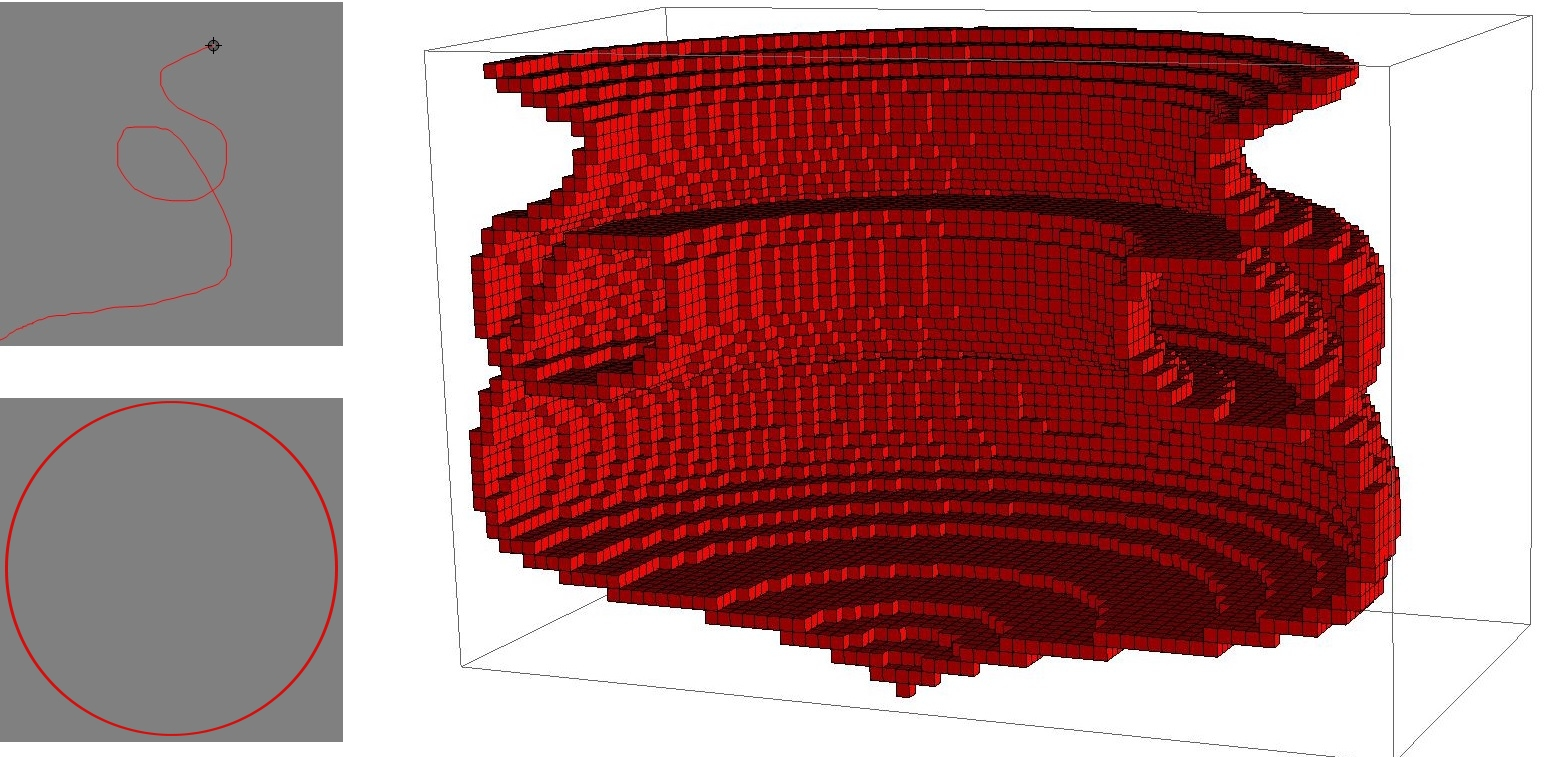
\includegraphics[height=3.8cm]{../Images/revolution2.jpg}
		\end{figure}
		\begin{itemize}
			\item Besoin d'un outil utilisable partout et par tous
		\end{itemize}
	\end{frame}
	

%---Objectifs------------------------------------------------------------------
	\subsection{Objectifs}
	\begin{frame}{\subsecname}
		\begin{itemize}
			\item Objectifs métiers
			\begin{itemize}
				\item Illustrer les r\'esultats de l'algorithme
				\item Mettre \`a disposition un outil de mod\'elisation
			\end{itemize}
		\end{itemize}
		\begin{itemize}
			\item Objectifs techniques
			\begin{itemize}
				\item Application web $\to$ WebGL
				\item Utilisable par tous
			\end{itemize}
		\end{itemize}
	\end{frame}


% --- Roles --------------------------------------------------------------------
	 \subsection{Organisation de l'\'equipe}
	 \begin{frame}{\subsecname}
		\begin{itemize}
			\item Composition de l'\'equipe~:
				\begin{itemize}
					\item Thomas \smallcaps{Benoist} - Chef de projet
					\item Zied \smallcaps{Ben} \smallcaps{Othmane} - Responsable qualit\'e
					\item Adrien \smallcaps{Bisutti} - Responsable des risques
					\item Lydie \smallcaps{Richaume} - Responsable des t\^aches
				\end{itemize}
		\end{itemize}
	\end{frame}




%===============================================================================
%	Cahier des charges
%===============================================================================

\section{Fonctionnalités demandées}
	\subsection{Génération des Surfaces}
	 \begin{frame}{\subsecname}
		\begin{itemize}
			\item Générer la surface
				\begin{itemize}
					\item A partir d'une méridienne et d'une courbe de révolution
					\item Méridienne : fonction y = f(x) ou paramétrique (dessin)
					\item Courbe de révolution : fonction implicite f(x,y) = 0
				\end{itemize}
		\end{itemize}
	\end{frame}


	\subsection{Gestion des courbes}
	 \begin{frame}{\subsecname}
		\begin{itemize}
			\item Afficher la méridienne et la courbe de révolution
			\item Pouvoir choisir la méridienne et la courbe de révolution de différentes façons :
				\begin{itemize}
					\item Choisir dans une liste de modèles
					\item Entrer une équation mathématique
					\item Dessiner une courbe (pour la méridienne)
				\end{itemize}
			\item Modifier les paramètres des modèles
			\item Afficher/cacher le repère des courbes
			\item Choisir la taille d'affichage des voxels
		\end{itemize}
	\end{frame}


	\subsection{Manipulation de l'espace 3D}
	 \begin{frame}{\subsecname}
		\begin{itemize}
			\item Choisir les dimensions
			\item Contrôler la caméra
			\item Mettre en évidence d'une méridienne et courbe de révolution sur la surface
			\item Choisir la connexité affichée
			\item Choisir la taille d'affichage des voxels
			\item Choisir des dimensions d'affichage de l'espace 3D (afficher des coupes)
			\item Afficher/cacher les limites de l'espace 3D
			\item Afficher/cacher l'objet repère
			\item Choisir vue orthographique/perspective
		\end{itemize}
	\end{frame}


	\subsection{Export et sauvegarde}
	 \begin{frame}{\subsecname}
		\begin{itemize}
			\item Exporter la surface générée :
				\begin{itemize}
					\item A destination d'un modeleur (format X3D)
					\item A destion d'une imprimante 3D (STL)
				\end{itemize}
			\item Exporter en PNG une image de la courbe de révolution, de la méridienne ou de la surface générée
			\item Sauvegarder les courbes dans une archive ZIP
			\item Charger les courbes à l'aide d'un ZIP générer par la fonction de sauvegarde
		\end{itemize}
	\end{frame}

	\subsection{Autre}
	\begin{frame}{\subsecname}
		\begin{itemize}
			\item Aide utilisateur
			\item Choix de la langue
			\item Sauvegarde automatique des courbes personnalisées dans le navigateur
		\end{itemize}
	\end{frame}

%===============================================================================
%	CONCLUSION
%===============================================================================

\section{Conclusion}


% --- Rappel -------------------------------------------------------------------
\begin{frame}{\secname}
	\begin{itemize}
		\item Organisation en cycles $\to$ d\'eveloppement incr\'emental
		\item Validation r\'egulière et avec les clients
		\item Un seul risque majeur
		\item Prochaine \'etape~: Conception
	\end{itemize}
\end{frame}


% --- Remerciment --------------------------------------------------------------
\begin{frame}{}
	\bigskip
	\bigskip
	\begin{titleblock}{}
		\begin{center}
			\smallskip
			\Large Surfaces de r\'evolution discrètes\\
			\medskip
			\small R\'eunion de lancement
			\smallskip
		\end{center}
	\end{titleblock}

	\bigskip
	\begin{center}
		Merci de votre attention.\\
		\medskip
		Avez-vous des questions\,?			
	\end{center}

	\bigskip
	\bigskip
	
\includegraphics[width=2cm]{../Images/logo-Xlim.png}
	\hfill
	
\includegraphics[width=2cm]{../Images/logo_univ_poitiers.png}
\end{frame}


\end{document}


